\documentclass[11pt,letter]{article}

\usepackage{graphicx}
\usepackage{float}

\usepackage{amsmath,amsfonts,amssymb}

\usepackage[inline]{enumitem}

\usepackage[margin=1in]{geometry}
\usepackage{longtable}
\renewcommand{\arraystretch}{3}
\usepackage{booktabs}
\usepackage{makecell}

\usepackage{blindtext}

\usepackage[dvipsnames]{xcolor}
\usepackage{listings}
\usepackage{textcomp}
\usepackage{verbatim}

\usepackage{hyperref}
\usepackage[capitalise]{cleveref}

\newcommand\myshade{85}
\colorlet{mylinkcolor}{violet}
\colorlet{mycitecolor}{YellowOrange}
\colorlet{myurlcolor}{Aquamarine}

\hypersetup{
  linkcolor  = mylinkcolor!\myshade!black,
  citecolor  = mycitecolor!\myshade!black,
  urlcolor   = myurlcolor!\myshade!black,
  colorlinks = true,
}

\lstdefinelanguage{Sandbox}
{
  basicstyle = \ttfamily,
  alsoletter = {-,?},
  morekeywords = [1]{rational, rational-polynomial, gain, derivative, integrate},
  keywordstyle = [1]\bfseries\color{green!50!black},
  morekeywords = [2]{pole-zero-plot, impulse-plot, step-plot, ramp-plot},
  keywordstyle = [2]\bfseries\color{blue!50!black},
  morekeywords = [3]{declare, transfer-function, zeros, poles,
    region-of-convergence, ?is, stable, convergent-at, LTIza, ask-ltiza},
  keywordstyle = [3]\bfseries,
  morekeywords = [4]{system, rat, rat-poly},
  keywordstyle = [4]\itshape,
  morekeywords = [5]{a,b,c,d,e,f,g,h,i,j,k,l,m,n,o,p,q,r,s,t,u,v,w,x,y,z,
    A,B,C,D,E,F,G,H,I,J,K,L,M,N,O,P,Q,R,S,T,U,V,W,X,Y,Z,
    alpha,beta,gamma,theta,tau,zeta},
  keywordstyle = [5]\underline,
  morekeywords = [6]{compose, feedback, parallel, sum},
  keywordstyle = [6]\bfseries\color{red!50!black},
  morecomment = [l]{;},
  commentstyle = \itshape\color{black!60!white},
  morestring = [b]",
  stringstyle = \color{green!50!blue},
}

\lstset{language=Sandbox,basicstyle=\ttfamily,tabsize=2,gobble=4,breaklines=True,upquote=True}

\title{An Embedded DSL for Simple Causal LTI Systems}
\author{T.~Mitchell~Roddenberry}
\date{25 March 2024}

\begin{document}

\maketitle

\begin{abstract}
  We present a simple domain-specific language (DSL) embedded in \texttt{Hy}, a LISP dialect that is itself embedded in \texttt{Python}.
  This DSL is designed for describing and analyzing rational causal LTI systems, with capabilities for symbolic expressions, variables, and plotting.
  The goal of this DSL is to provide an environment in which students can learn about basic properties of LTI systems experimentally, without needing to either
  \begin{enumerate*}[label=(\roman*)]
  \item learn an entire programming language syntax, or
  \item install heavy, proprietary, and overly-featureful simulation software.
  \end{enumerate*}

  The language strives to have syntax that is as simple as possible.
  It is of course not perfect in this regard.
  However, the hope in implementing this is to gradually improve the system to the point where users can operate it with what amounts to little more than colloquial language, much like the early LISP programs for expert systems.

  This manual begins with a tutorial, written in ``Q{\&}A" style,\footnote{Inspired heavily by Daniel P. Friedman and Matthias Felleisen. \emph{The Little Schemer}. MIT Press, 1995.} illustrating how the language works by example.
  Notably, the language is bundled with a chatbot that provides a ``natural language'' interface.
  For greater detail, the tutorial is followed by a technical reference on language features.
  See the appendices for information on installation.
\end{abstract}

\newpage

\tableofcontents

\newpage

\section{Tutorial}\label{sec:tutorial}

\begin{longtable}{ p{0.5\textwidth} p{0.5\textwidth} }
  \toprule
  \toprule
  What is \lstinline!s!?
  &
  \lstinline!s! is a \emph{symbol.} \\

  Are there any other symbols?
  &
  Yes, some of them include \lstinline!a , b , c , d , e , w , x , y , z!. \\

  Is that all of them?
  &
  No, symbols are also given by capital letters and the Greek alphabet. Examples include \lstinline!A , B , C , alpha , beta , gamma!. \\

  Which symbol is the most important?
  &
  All symbols are equal, but some are more equal than others. \lstinline!s! is the most equal symbol. \\

  Why is \lstinline!s! a special symbol?
  &
  Because we use it to represent the argument for the Laplace transform. \\

  Are there any other special symbols?
  &
  Yes, \lstinline!i! and \lstinline!j! represent $\sqrt{-1}$. \\

  \midrule
  \midrule
  What is \lstinline!'(system (rat 1 [] []))!?
  &
  It is a causal LTI system with a rational transfer function. \\

  Is it?
  &
  Ok, it is a \emph{representation} of a causal LTI system with a rational transfer function.
  See: \emph{The Treachery of Images}.
  We are not surrealists, nor are we French, so we will not distinguish between a system and its representation unless we have to. \\

  Does \lstinline!'(system (rat 1 [] []))! have any zeros?
  &
  No. \\

  Does \lstinline!'(system (rat 1 [] []))! have any poles?
  &
  No. \\

  What is the gain of \lstinline!'(system (rat 1 [] []))!?
  &
  The gain is $1$. \\

  So the transfer function of \lstinline!'(system (rat 1 [] []))! is $H(s)=1$?
  &
  Yes, that is correct. \\

  I am getting tired of writing down \lstinline!'(system (rat 1 [] []))!, is there a shorthand that I could use for this?
  &
  Yes, there are a few.
  Since it is a causal LTI system with no zeros or poles, it is determined only by its gain.
  The shorthand, then, is \lstinline!gain 1!, since it has a gain of $1$. \\

  What is \lstinline!(gain 2)! short for?
  &
  \lstinline!(gain 2)! is short for \lstinline!'(system (rat 2 [] []))!.\\

  \midrule

  \multicolumn{2}{c}{\Large\lstinline!gain! creates causal LTI systems that scale their input by a constant factor} \\

  \midrule

  Are there any other types of causal LTI systems with rational transfer functions?
  &
  Yes, of course there are. \\

  What is \lstinline!'(system (rat 1 [0] []))!?
  &
  It is a causal LTI system with a gain of $1$, a zero at $0$, and no poles. \\

  What is the transfer function of \lstinline!'(system (rat 1 [0] []))!?
  &
  It is $H(s)=s$. \\

  Woah, $H(s)$ looks like the symbol \lstinline!s!, right?
  &
  Good observation, I should have said that
  \begin{lstlisting}
    (transfer-function
      '(system
         (rat 1 [0] [])))
  \end{lstlisting}
  is \lstinline!s!. \\

  What does the system \lstinline!'(system (rat 1 [0] []))! do?
  &
  It is a system that takes the derivative of its input. \\

  Is there a shorthand for \lstinline!'(system (rat 1 [0] []))!?
  &
  Yes, \lstinline!(derivative)! is shorthand for \lstinline!'(system (rat 1 [0] []))!. \\

  What is the opposite of differentiation?
  &
  Integration. \\

  What is the gain of a causal LTI system that integrates its input?
  &
  The gain of such a system is $1$. \\

  Does the transfer function of a causal LTI system that integrates its input have any zeros?
  &
  No. \\

  Does the transfer function of a causal LTI system that integrates its input have any poles?
  &
  Yes, it has a pole at $0$. \\

  Is \lstinline!'(system (rat 1 [] [0]))! a causal LTI system that integrates its input?
  &
  Yes; a piece of shorthand for it is \lstinline!(integrate)!. \\

  \midrule

  \multicolumn{2}{c}{\Large\lstinline!derivative , integrate! create causal LTI systems} \\

  \midrule

  What happens if I say \lstinline!(declare S gain 2)!?
  &
  It creates \lstinline!(gain 2)!, but we have given it the name \lstinline!S!. \\

  After that, what happens if I type in \lstinline!S!?
  &
  You will get \lstinline!(gain 2)! back. \\

  How would I create a differentiator denoted by \lstinline!D!?
  &
  \lstinline!(declare D derivative)! \\

  Does \lstinline!(declare I integrate)! create an integrator named \lstinline!I!?
  &
  Yes, it does. \\

  But \lstinline!S , D , I! are symbols, are they not?
  &
  That is true, but \lstinline!declare! renames them. \\

  Can I \lstinline!(declare s gain 1)!?
  &
  You could, but I would not suggest it! \\

  \midrule

  \multicolumn{2}{c}{\Large\lstinline!declare! is a prefix that names systems} \\

  \midrule

  What if I want to put systems together?
  &
  Sure, what do you have in mind? \\

  I would like to make a system that takes a derivative, then scales by a factor of $2$.
  &
  Ok, so you would like to put a \lstinline!(derivative)! and a \lstinline!(gain 2)! in series? \\

  Yes! How do I do that?
  &
  \lstinline!(compose (derivative) (gain 2))!. \\

  What LTI system is that?
  &
  \begin{lstlisting}
    ['compose '(system
                 (rat 1 [0] []))
              '(system
                 (rat 2 [] []))]
  \end{lstlisting} \\

  Can I give that system a name?
  &
  Sure, just use \lstinline!declare!. \\

  Like this?
  \begin{lstlisting}
    (declare diffscale compose
                         (derivative)
                         (gain 2))
  \end{lstlisting}
  &
  Excellent. \\

  Are there other ways to combine systems?
  &
  Yes, you can put systems in parallel using \lstinline!parallel! or \lstinline!sum!, and you can create feedback systems using \lstinline!feedback!. \\

  Explain \lstinline!parallel! to me.
  &
  \lstinline!(parallel S1 S2)! creates an LTI system that applies \lstinline!S1\lstinline and \lstinline!S2! to the input, then sums the respective output. \\

  Tell me the transfer function of
  \begin{lstlisting}
    (parallel (derivative) (integrate))
  \end{lstlisting}
  &
  \lstinline!s + 1/s! \\

  Does \lstinline!sum! behave any differently?
  &
  No. \\

  How many systems can I put in parallel using \lstinline!parallel!?
  &
  As many as you want: \lstinline!(parallel S1 S2 S3)! is valid syntax. \\

  Some systems have feedback loops, can I create those?
  &
  Yes, use \lstinline!(feedback S1 S2)!. \\

  Tell me the transfer function of
  \begin{lstlisting}
    (feedback (gain 2) (integrate))
  \end{lstlisting}
  &
  \lstinline!2/(1+2/s)! \\

  How many systems can I apply feedback to?
  &
  Only two: but those systems can each consist of \emph{composed, parallel,} or \emph{feedback} systems themselves! \\

  \midrule

  \multicolumn{2}{c}{\Large\lstinline!compose , parallel , feedback! combine LTI systems} \\

  \midrule

  Typing some of these things in is a bit tedious: show me how to make a complicated system out of systems that I have already named.
  &
  Use the names as shorthand:
  \begin{lstlisting}
    (declare S1 gain 2)
    (declare S2 derivative)
    (declare S3 integrate)
    (declare S4 feedback (compose S1 S2) S3)
  \end{lstlisting} \\

  What is the transfer function of this system?
  &
  You can find it like this:
  \begin{lstlisting}
    (transfer-function S4)
  \end{lstlisting}
  %
  is \lstinline!2*s/3!. \\

  Is there a one-liner for defining \lstinline!S4! like above, while also naming the systems \lstinline!S1,S2,S3!?
  &
  Like this?
  \begin{lstlisting}
    (declare S4 feedback
      (compose (declare S1 gain 2)
               (declare S2 derivative))
      (declare S3 integrate))
  \end{lstlisting} \\

  \midrule

  \multicolumn{2}{c}{\Large Use \lstinline!declare! statements to name things along the way} \\

  \midrule

  All of the systems we have built so far only have poles and zeros at $0$.
  &
  That is correct. \\

  What is the gain of \lstinline!'(system (rat 2 [] [3]))!?
  &
  $2$ \\

  What are the zeros of \lstinline!'(system (rat 2 [] [3]))!?
  &
  There are none. \\

  What are the poles of \lstinline!'(system (rat 2 [] [3]))!?
  &
  There is a single pole at $3$. \\

  What is \lstinline!(rational 2 [] [3])!?
  &
  \lstinline!'(system (rat 2 [] [3]))! \\

  What are the zeros of \lstinline!'(system (rat 3 [1+1j 1-1j] []))!?
  &
  There is are two zeros at $1\pm j$, where $j=\sqrt{-1}$. \\

  What is \lstinline!(rational 3 [1+1j 1-1j] [])!?
  &
  \lstinline!'(system (rat 3 [1+1j 1-1j] []))! \\

  Neat, so \lstinline!rational! creates causal LTI systems with rational transfer functions from their gain, zeros, and poles.
  &
  You got it! \\

  What if I know the numerator and denominator of the transfer function, but not the gain, poles, and zeros?
  &
  Use \lstinline!rational-polynomial!. \\

  What is \lstinline!(rational-polynomial "2*s**2-2*s+2" "s+1")!?
  &
  \lstinline!'(system (rat-poly 2*s**2-2*s+2 s+1))!. \\

  What is the transfer function of \lstinline!'(system (rat-poly 2*s**2-2*s+2 s+1))!?
  &
  The transfer function can be computed as follows.
  \begin{lstlisting}
    (transfer-function '(system
                          (rat-poly
                            2*s**2-2*s+2
                            s+1)))
  \end{lstlisting}
  is \lstinline!(2*s**2-2*s+2)/(s+1)!.\\

  \midrule

  \multicolumn{2}{c}{\Large\lstinline!rational , rational-polynomial! create LTI systems} \\

  \midrule

  What does \lstinline!(declare S1 rational 1 [1] [-1])! do?
  &
  Names \lstinline!S1! as an LTI system with gain $1$, a zero at $1$, and a pole at $-1$. \\

  Is \lstinline!S1! stable?
  &
  Good question.
  \begin{lstlisting}
    (?is S1 stable)
  \end{lstlisting}
  yields \lstinline!True!, so yes. \\

  Why is it stable?
  &
  Because its region of convergence contains the imaginary axis. \\

  Are you sure?
  &
  Yes.
  \begin{lstlisting}
    (region-of-convergence S1)
  \end{lstlisting}
  yields \lstinline!re(s)>-1!. \\

  Can you check the convergence of the Laplace transform at $1+j$?
  &
  Sure.
  \begin{lstlisting}
    (?is S1 convergent-at 1+1j)
  \end{lstlisting}
  yields \lstinline!True!. \\

  What are the zeros of \lstinline!S1!?
  &
  Try the command
  \begin{lstlisting}
    (zeros S1)
  \end{lstlisting}
  which yields \lstinline![1]!. \\

  What are the poles of \lstinline!S1!?
  &
  Similarly,
  \begin{lstlisting}
    (poles S1)
  \end{lstlisting}
  yields \lstinline![-1]!. \\

  \midrule

  \multicolumn{2}{c}{\Large Ask questions with \lstinline!?is!} \\

  \midrule

  What is the pole-zero plot of the system declared below?
  \begin{lstlisting}
    (declare S1 feedback
                (rational 1 [1] [-2])
                (compose (integrate)
                         (gain -1)))
  \end{lstlisting}
  &
  \lstinline!(pole-zero-plot S1)! displays the figure below:
  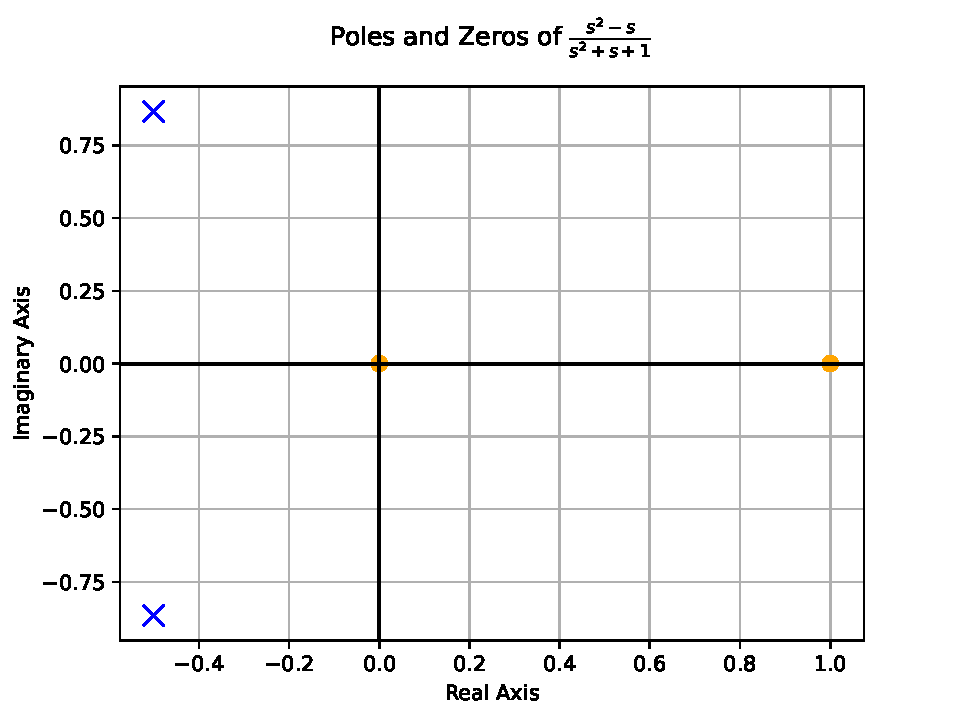
\includegraphics[width=\linewidth]{figs/pz-feedback} \\

  Is \lstinline!S1! stable?
  &
  Yes: \lstinline!(?is S1 stable)! yields \lstinline!True!. \\

  Does this make sense?
  &
  Yes, the poles are to the left of the imaginary axis.
  \begin{lstlisting}
    (region-of-convergence S1)
  \end{lstlisting}
  yields \lstinline!re(s) > -1/2!. \\

  Is the computer smart enough to cancel out poles and zeros that overlap?
  &
  Yes! But it may be subject to numerical error, so be careful.\\

  What is the impulse response of \lstinline!S1!?
  &
  You can plot it with \lstinline!(impulse-plot S1)!
  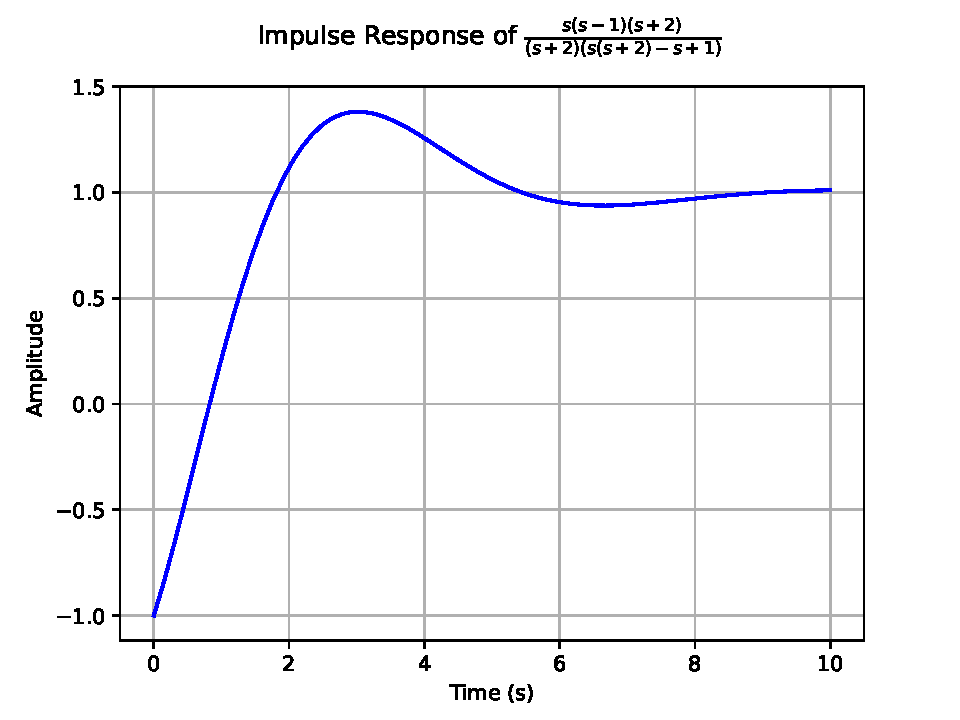
\includegraphics[width=\linewidth]{figs/impulse-feedback} \\

  What if the impulse response isn't well-defined?
  &
  Then you should try \lstinline!(step-plot S1)! or \lstinline!(ramp-plot S1)!. \\

  Can I see the impulse response for $20$ seconds?
  &
  Yes, specify with \lstinline!(impulse-plot S1 :upper-limit 20)!.
  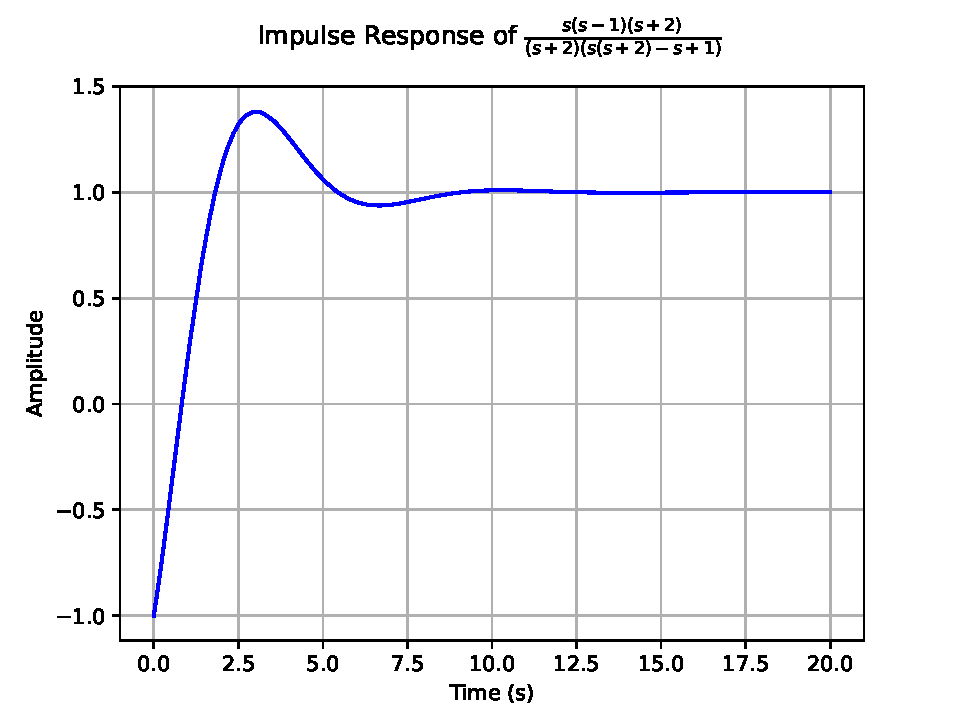
\includegraphics[width=\linewidth]{figs/impulse-feedback-2} \\

  \midrule

  \multicolumn{2}{c}{\Large Visualize with \lstinline!pole-zero-plot , impulse-plot , step-plot , ramp-plot!} \\

  \midrule

  What is the transfer function of \lstinline!(rational 1 [] [a])!?
  &
  \lstinline!(transfer-function (rational 1 [] [a]))! is \lstinline!1/(s-a)!. \\

  What is the pole-zero plot of the system declared below?
  \begin{lstlisting}
    (declare S1 rational 1 [a] [b])
  \end{lstlisting}
  &
  There is not enough information to tell. \\

  What is the pole-zero plot when $a=1$ and $b=-1$?
  &
  Let us take a look. \lstinline!(pole-zero-plot S1 {a 1 b -1})! yields
  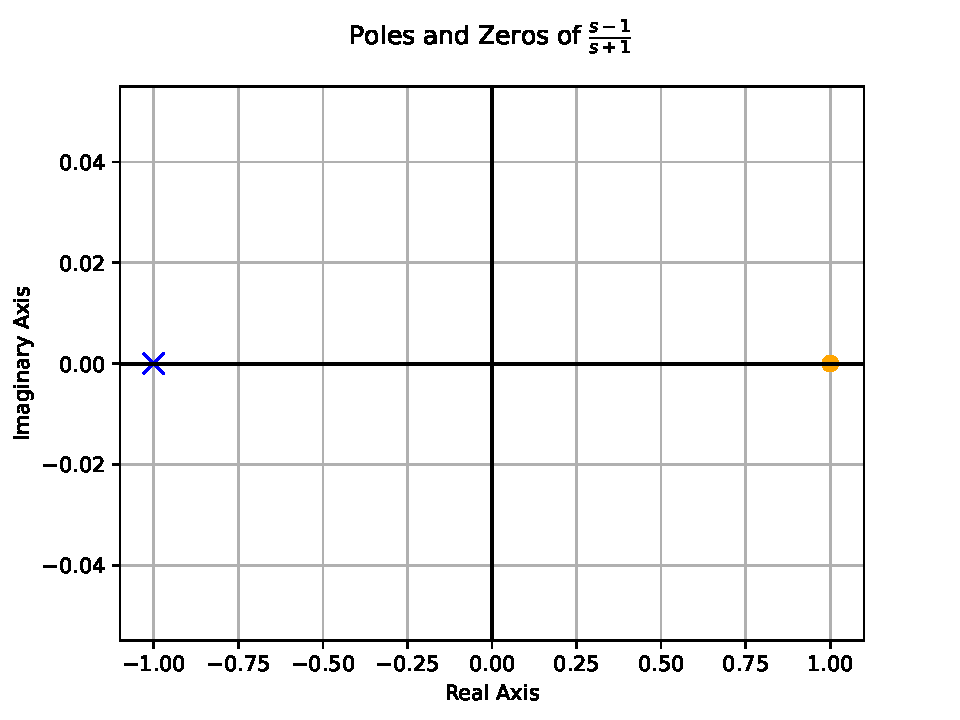
\includegraphics[width=\linewidth]{figs/pz-bind} \\

  What are the zeros of \lstinline!S1!?
  &
  \lstinline!(zeros S1)! yields \lstinline![a]!. \\

  What are the zeros of \lstinline!S1! when $b=1$?
  &
  \lstinline!(zeros S1 {b 1})! yields \lstinline![a]!. \\

  What are the poles of \lstinline!S1! when $b=-1$?
  &
  \lstinline!(poles S1 {b -1})! yields \lstinline![-1]!. \\

  What is the region of convergence of \lstinline!S1!?
  &
  \lstinline!(region-of-convergence S1)! yields \lstinline!re(s)>re(b)!. \\

  Is the Laplace transform of \lstinline!S1! convergent at $s=b+1$?
  &
  Yes: \lstinline!(?is S1 convergent-at (+ b 1))! yields \lstinline!True!. \\

  \midrule

  \multicolumn{2}{c}{\Large When there are degrees of freedom, bind symbols with \lstinline!\{...\}!} \\

  \midrule

  What are the poles of the system declared below?
  \begin{lstlisting}
    (declare S1 rational 1 [] [a])
  \end{lstlisting}
  &
  \lstinline!(poles S1)! yields \lstinline!a!. \\

  \lstinline!(?is S1 stable)!
  &
  \lstinline!re(a) < 0!
  \\

  What is \lstinline!(region-of-convergence S1)!?
  &
  \lstinline!re(s) > re(a)!
  \\

  Is \lstinline!S1! stable when $a=1$?
  &
  How do you think we should see? \\

  Like this maybe? \lstinline!(?is S1 {a 1} stable)!
  &
  That won't work. You need to use special syntax when using \lstinline!?is!.
  \begin{lstlisting}
    (?is S1 stable :bind {a 1})
  \end{lstlisting} \\

  Ahh, ok, \lstinline!:bind! tells us what \lstinline!{a 1}! does.
  &
  Right, you need to be sure to use \lstinline!:bind! whenever you combine \lstinline!?is! and symbolic expressions. \\

  \midrule

  \multicolumn{2}{c}{\Large When using \lstinline!?is!, bind symbols with \lstinline!:bind \{...\}!} \\

  \midrule

  What are the poles of the system declared below?
  \begin{lstlisting}
    (declare S1 rational 1 [a] [a b c])
  \end{lstlisting}
  &
  \lstinline!(poles S1)! yields \lstinline![b c]!. \\

  What is the region of convergence of \lstinline!S1!?
  &
  \lstinline!(region-of-convergence S1)! yields \lstinline!re(s) > Max(re(b), re(c))!. \\

  \lstinline!(?is S1 stable :bind {c (+ b 1)})!
  &
  \lstinline!re(b) + 1 < 0! \\

  \midrule

  \bottomrule

\end{longtable}

\subsection{Exercise}\label{sec:tutorial:exercise}

\noindent\textbf{Problem:} Construct a feedback system using a single-pole filter and constant-gain feedback.
%
\begin{enumerate}
\item Determine the transfer function.
\item Determine the poles and zeros in terms of the gain of the filter, the pole of the filter, and the gain of the feedback system.
  \begin{enumerate}
  \item Determine a set of parameters such that the system is stable, then plot the poles and zeros.
  \item Determine a set of paramaters such that the system is unstable, then plot the poles and zeros.
  \end{enumerate}
\item Is the system stable when the filter has gain $1$ and a pole at $1$, and the feedback has a gain of $2$?
  \begin{enumerate}
  \item If so, plot the impulse response.
  \item If not, plot the step response.
  \end{enumerate}
\item Is the system stable when the pole of the filter is equal to the product of the gain of the filter and the gain of the feedback? What about when it is equal to the product of the gains minus one?
\end{enumerate}

\newpage
\noindent \textbf{Solution:}

\lstinputlisting[numbers=left,title=\lstname]{exercise1.lti}

\newpage
\noindent \textbf{Program output:}

\verbatiminput{output1.txt}

\begin{figure}[H]
  \centering
  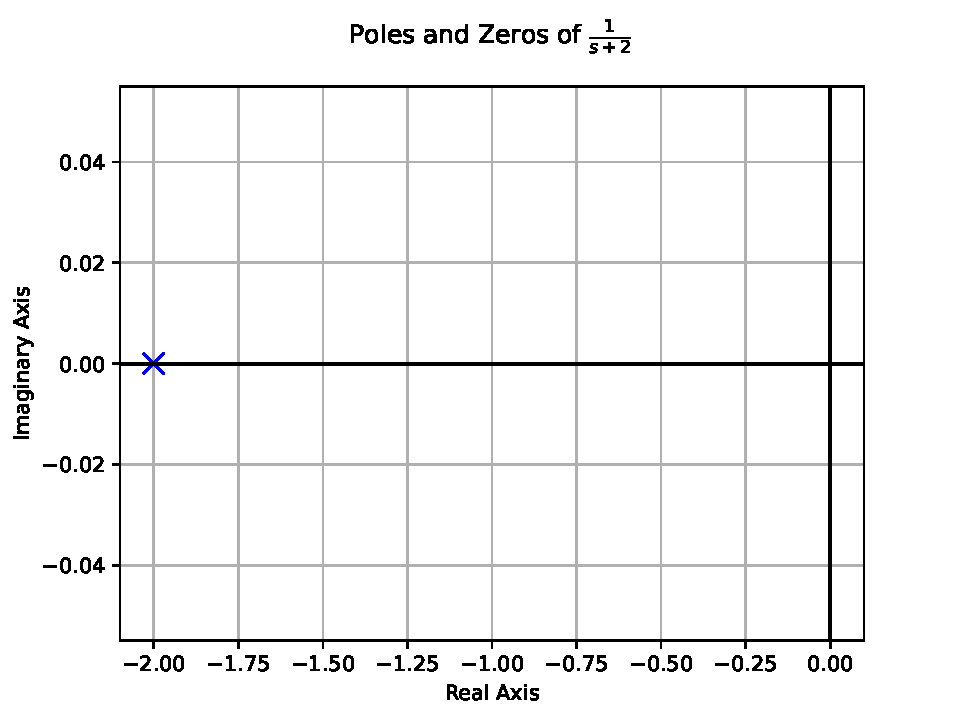
\includegraphics[width=0.3\linewidth]{figs/ex1-stable-pz}
  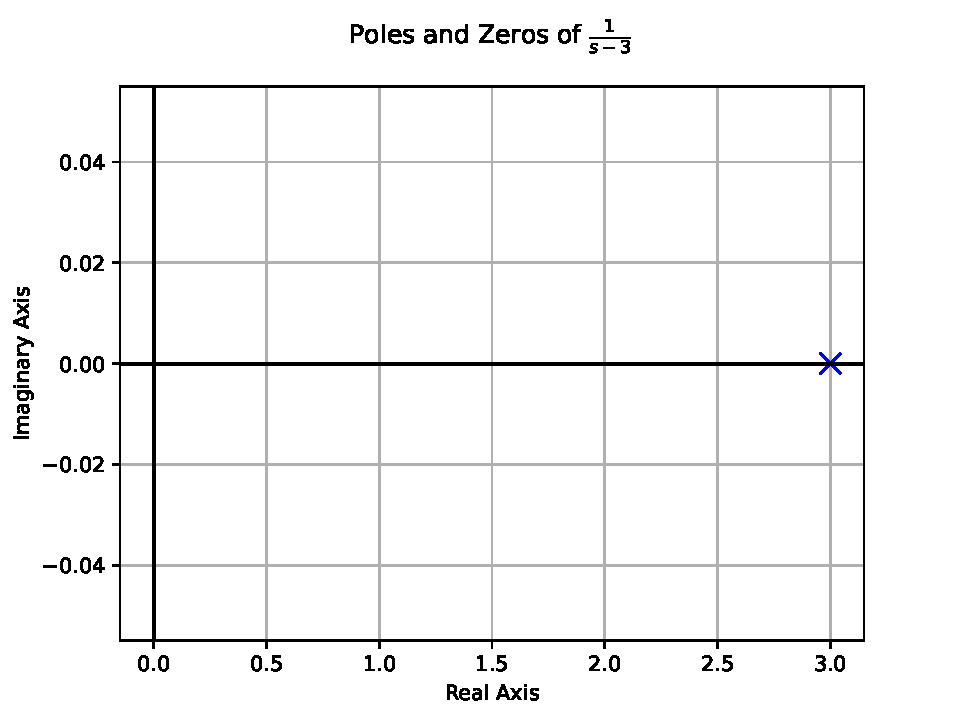
\includegraphics[width=0.3\linewidth]{figs/ex1-unstable-pz}
  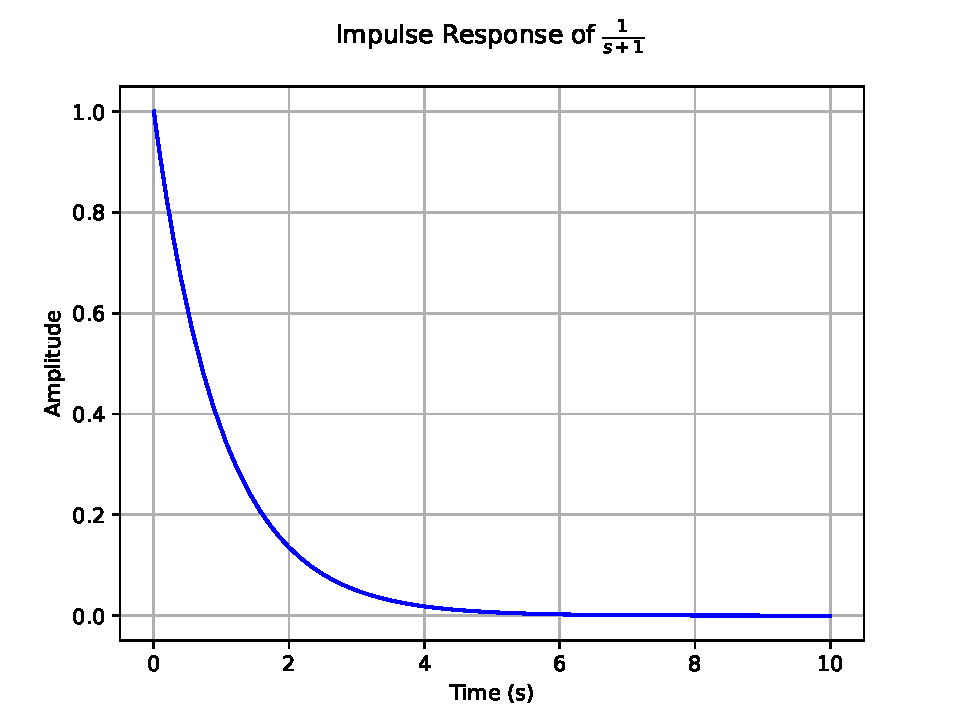
\includegraphics[width=0.3\linewidth]{figs/ex1-response}
  \caption{Plots for first exercise. Parts 2a, 2b, and 3 from left to right, respectively.}
\end{figure}

\newpage

\subsection{LTIza: A Helpful Chatbot}

\lstinline!ELIZA! is a famous chatbot\footnote{Originally called ``chatterbots.''} written by Joseph Weizenbaum in the 1960s, capable of simulating Rogerian psychobabble via simple pattern matching rules.
For those who are averse to learning programming language syntax, such as the one demonstrated earlier, a simple chatbot named \lstinline!LTIza! is provided.

To start a conversation with \lstinline!LTIza!, you need to be in an interactive session and have a system declared with some name, say \lstinline!S1!.
Then, run the command \lstinline!(ask-ltiza S1)! to enter a REPL.\footnote{Read-evaluate-print loop: the usual interactive interface for shell-like programs.}
Within the \lstinline!LTIza! REPL, you can give a variety of loosely-structured queries, which the program will then attempt to parse into a command.
If the command is a ``verb,'' so-to-speak, then it will print the command and run it.
If the command defines a ``noun,'' in particular if it binds symbols to values, then it will show the set of bound symbols in the prompt.
See below for an example session.

\begin{lstlisting}[gobble=2]
  => (declare S1 rational 1 [a] [-2 -1 b])
  => (ask-ltiza S1)
  LTIza {} => what are the poles
    (poles S {})
    [-2, -1, b]
  LTIza {} => what are the zeros
    (zeros S {})
    [a]
  LTIza {} => bind a equal to -3
  LTIza {a: -3} => bind b to 1
  LTIza {a: -3, b: 1} => poles
    (poles S {a -3 b 1})
    [-3, -2, -1]
  LTIza {a: -3, b: 1} => is the system stable
    (stable S {a -3 b 1})
    True
  LTIza {a: -3 b: 1} => unbind a
  LTIza {b: 1} => what is the region of convergence
    (region-of-convergence S {b 1})
    re(s) > Max(-2, re(a))
  LTIza {b: 1} => is the system stable
    (stable S {b 1})
    re(a) < 0
  LTIza {b: 1} => quit
  =>
\end{lstlisting}

You can type \lstinline!help! at the \lstinline!LTIza {} =>! prompt to get more information about available functionality.
Be encouraged by this tool: use the code output to learn how to write your own programs in more formal language!

\section{Reference}

\subsection{Language Core}

The core language features can be found in \lstinline!systems_sandbox.hy!.

\subsubsection{Defining Systems}

\begin{longtable}{ p{0.6\textwidth} p{0.4\textwidth} }
  \texttt{(rational [[gain 1]] [zeros []] [poles []])}
  &
  Returns a representation of a causal LTI system with rational transfer function of the form
  \begin{equation*}
    H(s) = \frac{\mathrm{gain}\times\prod_{z\in\mathrm{zeros}}(s-z)}{\prod_{p\in\mathrm{poles}}(s-p)}.
  \end{equation*}
  \texttt{gain} is a numeric value or a symbol, \texttt{zeros} is a list of numeric values or symbols, and \texttt{poles} is a list of numeric values or symbols.
  \\

  \texttt{(rational-polynomial [[numerator 1] [denominator 1]])}
  &
  Returns a representation of a causal LTI system with transfer function of the form
  \begin{equation*}
    H(s) = \frac{\mathrm{numerator}}{\mathrm{denominator}}.
  \end{equation*}
  \texttt{numerator,denominator} are strings coinciding with a polynomial of numerics and symbols.
  \\

  \texttt{(gain [[gain 1]])}
  &
  Alias for \texttt{(rational gain)}. \\

  \texttt{(derivative [])}
  &
  Alias for \texttt{(rational 1 [0] [])}. \\

  \texttt{(integrate [])}
  &
  Alias for \texttt{(rational 1 [] [0])}. \\

  \texttt{(compose [\#* l])}
  &
  Composes multiple systems in series. Takes a variable number of arguments. \\

  \texttt{(feedback [S T])}
  &
  Creates a feedback system from two systems. \\

  \texttt{(parallel [\#* l])}
  &
  Combines multiple systems in parallel. Takes a variable number of arguments. \\

  \texttt{(sum [\#* l])}
  &
  Same as \texttt{parallel}. \\

  \texttt{(declare [S \#* H])}
  &
  Macro to assign whatever expression is given by \texttt{H} to the name \texttt{S}.
  Note: \texttt{H} should not be enclosed by parentheses, \textit{e.g.}, \texttt{(declare S gain 2)}. \\

\end{longtable}

\subsubsection{System Analysis}

\begin{longtable}{ p{0.6\textwidth} p{0.4\textwidth} }
  \texttt{(transfer-function [S [bind \{\}]])}
  &
  Displays the transfer function of the system \texttt{S} after binding symbols according to the dictionary \texttt{bind}. \\

  \texttt{(zeros [S [bind \{\}]])}
  &
  Returns the zeros of the system \texttt{S} after binding symbols according to the dictionary \texttt{bind}. \\

  \texttt{(poles [S [bind \{\}]])}
  &
  Returns the poles of the system \texttt{S} after binding symbols according to the dictionary \texttt{bind}. \\

  \texttt{(region-of-convergence [S [bind \{\}]])}
  &
  Returns inequality expressing values of symbol \texttt{s} for which the transfer function of the system \texttt{S} is convergent, after binding symbols according to the dictionary \texttt{bind}. \\

  \texttt{(stable [S [bind \{\}]])}
  &
  After binding symbols according to the dictionary \texttt{bind}, either returns Boolean (True/False) value indicating if the system \texttt{S} is stable, or returns inequality indicating conditions underwhich \texttt{S} is stable if there are remaining degrees of freedom.
\end{longtable}

\subsubsection{Plotting}

\begin{longtable}{ p{0.6\textwidth} p{0.4\textwidth} }
  \texttt{(pole-zero-plot [S [bind \{\}]] \#** kwargs)}
  &
  Plots the pole-zero plot of the system \texttt{S} after binding symbols according to the dictionary \texttt{bind}.
  Passes \texttt{kwargs} to plotting function. \\

  \texttt{(impulse-plot [S [bind \{\}]] \#** kwargs)}
  &
  Plots the impulse response of the system \texttt{S} after binding symbols according to the dictionary \texttt{bind}.
  Passes \texttt{kwargs} to plotting function. \\

  \texttt{(step-plot [S [bind \{\}]] \#** kwargs)}
  &
  Plots the step response of the system \texttt{S} after binding symbols according to the dictionary \texttt{bind}.
  Passes \texttt{kwargs} to plotting function. \\

  \texttt{(ramp-plot [S [bind \{\}]] \#** kwargs)}
  &
  Plots the ramp response of the system \texttt{S} after binding symbols according to the dictionary \texttt{bind}.
  Passes \texttt{kwargs} to plotting function. \\

  \texttt{(frequency-plot [S [bind \{\}] [sigma0 0]] \#** kwargs)}
  &
  After binding symbols according to the dictionary \texttt{bind}, plots the magnitude of the transfer function of the system \texttt{S} at $H(\sigma_0+j\omega)$ for varying values of $\omega$.
  Passes \texttt{kwargs} to plotting function.
\end{longtable}

\newpage

\appendix

\section{Installation \& Getting Started}

At this point, I haven't packaged this software in a slick way -- it relies on the user having a working Python 3 installation and being able to install the required packages via \texttt{pip} or some other means.
For now, you should just run the included script \texttt{main.py} from within the project directory.
If I get around to it, I'll figure out a good way to package everything.

\subsection{Prerequisites}

This program was developed with \texttt{Python 3.11.8}, but it will probably work fine on earlier version of \texttt{Python 3.11}, and even on \texttt{Python 3.9} or \texttt{Python 3.10}.
No promises, though.

You will also need a \texttt{pip} installation alongside your \texttt{Python} install.
Chances are that \texttt{pip} was distributed with \texttt{Python}.

The rest of the installation tutorial will use ``virtual environments,'' another feature that comes with \texttt{Python}.

\subsection{Installation}

The left column of the instructions describes what you are doing, and the right column shows it in a terminal\footnote{In particular, a shell like \texttt{bash} or \texttt{sh}. I don't know anything about using Windows.} session.
The \texttt{\$} at the beginning of each line refers to the terminal prompt.
You should not type it in yourself.

\begin{longtable}{ p{0.4\textwidth} p{0.6\textwidth} }
  Navigate to the directory where you have downloaded the source code.
  For me, that directory is called \texttt{elec242}, and I obtain the source code via \texttt{git}.
  You may wish to get the source code some other way; that's fine.
  &
  \begin{lstlisting}[language=bash]
    $ git clone https://github.com/tmrod/systems-sandbox ~/elec242
    $ cd ~/elec242
  \end{lstlisting}
  \\

  Create a virtual environment in that directory, then activate it.
  &
  \begin{lstlisting}[language=bash]
    $ python -m venv .venv
    $ . ./.venv/bin/activate
  \end{lstlisting}
  \\

  With the virtual environment activated, you may or may not see a change in your prompt.
  Either way, continue on to install the necessary packages.
  &
  \begin{lstlisting}[language=bash]
    (venv)$ pip install -r requirements.txt
  \end{lstlisting}
\end{longtable}

Hopefully that worked.
Congratulations: you have now installed everything you need!

\subsection{Getting Started}

\begin{longtable}{ p{0.4\textwidth} p{0.6\textwidth} }
  I'll assume that you followed the instructions from the previous section.
  Navigate to the directory where you installed everything and activate the virtual environment.
  &
  \begin{lstlisting}[language=bash]
    $ cd ~/elec242
    $ . ./venv/bin/activate
    (venv) $
  \end{lstlisting}
  \\

  To start up a REPL, run the script \texttt{main.py} with no arguments.
  Be sure that you run this \emph{from the install directory}.
  Once again, I haven't bothered to package the program files in a way that is convenient.
  This will drop you into a REPL.
  The startup banner might vary depending on your particular system.
  &
  \begin{lstlisting}[language=bash]
    (venv) $ python main.py
    Hy 0.27.0 using CPython(main) ...
    =>
  \end{lstlisting}
  \\

  The prompt \texttt{=>} corresponds to the REPL in which you can type in commands to describe and study systems.
  This is a good time to start working through \cref{sec:tutorial}.
  For instance, you could declare a system, then ask the chatbot about it.
  &
  \begin{lstlisting}[language=bash]
    => (declare S1 rational 1 [a] [-2 -1 b])
    => (ask-ltiza S1)
    LTIza {} => what are the poles
      (poles S {})
      [-2, -1, b]
    LTIza {} => quit
  \end{lstlisting}
  \\

  And to exit the REPL, \texttt{<Ctrl+d>} works.
  &
  \begin{lstlisting}[language=bash]
    => <Ctrl+d>
    (venv) $
  \end{lstlisting}
  \\

  In \cref{sec:tutorial:exercise}, we put the solution to a question in a file and ran it all at once, rather than typing each command manually at the REPL.
  Suppose there is some file containg commands, say, at \texttt{manual/exercise1.lti}.
  It can be run like this:
  &
  \begin{lstlisting}[language=bash]
    (venv) $ python main.py manual/exercise1.lti
    1. Transfer function is:  TransferFunction(b, -a + b*k + s, s)
    2. Poles:  [a - b*k]
    2. Zeros:  []
    RoC:  re(s) > re(a) - re(b*k)
    2a. Is {a=1, b=1, k=3} stable?  True
    2b. Is {a=1, b=1, k=-2} stable?  False
    3. {a=1, b=1, k=2} is stable.
    4. Is {a=b*k} stable?  False
    4. Is {a=b*k-1} stable?  True
  \end{lstlisting}
  \\

  Notice: at the top of the script there are two important lines.
  When running a file as a script like this, you need to include those to make everything work.
  I'll figure out how to remove the need for those once I package this software properly.
  &
  \begin{lstlisting}
    (import systems_sandbox *)
    (require systems_sandbox *)
  \end{lstlisting}
\end{longtable}

\end{document}
